\documentclass{article}

% if you need to pass options to natbib, use, e.g.:
\PassOptionsToPackage{numbers, compress}{natbib}
% before loading neurips_2024


% ready for submission
\usepackage{neurips_2024}


% to compile a preprint version, e.g., for submission to arXiv, add add the
% [preprint] option:
    % \usepackage[preprint]{neurips_2024}


% to compile a camera-ready version, add the [final] option, e.g.:
    % \usepackage[final]{neurips_2024}


% to avoid loading the natbib package, add option nonatbib:
    % \usepackage[nonatbib]{neurips_2024}


\usepackage[utf8]{inputenc} % allow utf-8 input
\usepackage[T1]{fontenc}    % use 8-bit T1 fonts
\usepackage{hyperref}       % hyperlinks
\usepackage{url}            % simple URL typesetting
\usepackage{booktabs}       % professional-quality tables
\usepackage{amsfonts}       % blackboard math symbols
\usepackage{nicefrac}       % compact symbols for 1/2, etc.
\usepackage{microtype}      % microtypography
\usepackage{xcolor}         % colors
\usepackage{graphicx}       % include graphics


\title{Second Paper Summary, EE245 Spring 2025}

\author{%
  Kunyi Yu \\
  Department of Computer Science and Engineering \\
  University of California, Riverside \\
  Riverside, CA 92507 \\
  \texttt{kyu135@ucr.edu} \\
}

\begin{document}

% pdflatex main.tex; bibtex main; pdflatex main.tex; pdflatex main.tex

\maketitle

\begin{abstract}
  The second paper summary due on Monday, May 19, 2025. The author chose the paper titled "\underline{Benchmarking Safe Exploration in Deep Reinforcement Learning}" by Alex Ray, Joshua Achiam, and Dario Amodei from OpenAI.

  % The following content covers 1) major contributions, 2) prior work, 3) method, 4) major results, 5) strengths, and 6) weaknesses.
\end{abstract}

% Components (2-3 pages)
% 1. Summary of major contributions – 15%
% 2. Relation to prior work – 15%
% 3. Summary of the method – 20%
% 4. Summary of major results – 20%
% 5. Summary of strengths – 15%
% 6. Summary of weaknesses – 15%

\section{Summary of Major Contributions}

When training a reinforcement learning (RL) agent interacting with human, it is crucial to ensure a safe exploration. Otherwise, the agent may take actions that are harmful to human or the environment, such as autonomous vehicles accidents, AI systems causing power grid failures, or question-answering systems generating misleading medical advice. As a result, the paper \cite{ray2019benchmarking} advance the study of it by proposing three major contributions:

First, the authors propose to standardize constrained RL to be the major formalism for safe exploration. They argue that safety specifications are indipendent of the performance specifications, and constrained RL is a natural way to formalize this. The authors also note that the constrained RL is scalable to high-dimensional methods.

Second, the paper provides the Safety Gym benchmark suite consisting of 18 high-dimensional continuous control tasks for safe exploration, 9 tasks for debugging, and tools for building extensive environments. They claim each environment express task performance and safety via a reward function and a set of additional cost functions. Moreover, Safety Gym has different levels of difficulty, randomized initial states, and highly extensive environments.


Finally, the authors establish a set of baselines for both unconstrained RL algorithms such as Trust Region Policy Optimization (TRPO) \cite{schulman2015trust} and Proximal Policy Optimization (PPO) \cite{schulman2017proximal}, and constrained RL algorithms such as Lagrangian methods, Constrained Policy Optimization (CPO) \cite{achiam2017constrained}, and a constrained version of TRPO. They found that the performance of CPO is poor compared to Lagrangian methods.

\section{Relation to Prior Work}

Three aspects of prior work are reviewed in Section 2 of the paper:

\textbf{Safety Overviews}: \citet{amodei2016concrete} and \citet{leike2017ai} provide two taxonomies and examples of safety problems in AI, including safe exploration. Two additional surveys discuss non-learning approaches to safety, which are omitted here because the paper focuses on modern deep RL methods.

\textbf{Safety Definitions and Algorithms}: The paper mentions 13 safety definitions or their variations, including: labeling states of environments as ``safe'' or ``unsafe'' \cite{hans2008safe}, which is often related to constraints \cite{haviv1996constrained}; considering agents to be safe if they act, reason, and generalize within human preferences \cite{hadfield2016cooperative, christiano2017deep, irving2018ai, leike2018scalable}; and so on.

The mentioned RL algorithms include: using ensembles to learn generalized safe policies \cite{kenton2019generalizing}; preventing unsafe actions by learning action-time interventions \cite{dalal2018safe, chow2019lyapunov}; using human interventions to avoid unsafe actions \cite{saunders2017trial}; and so on.

\textbf{Benchmarking RL and RL Safety}: The paper mentions several general RL benchmarks, including: ALE \cite{bellemare2013arcade}, OpenAI Gym \cite{brockman2016openai}, DeepMind Control Suite \cite{tassa2018deepmind}, MuJoCo simulator \cite{todorov2012mujoco}, and CoinRun \cite{cobbe2019quantifying}. Unlike these general RL benchmarks, \citet{leike2017ai} provide grid worlds demonstrating AI safety problems by using dueling reward functions evaluating both performance and safety.

Section 3 of the paper introduces several basic concepts. An optimal policy in \textbf{Constrained RL} is given by $\pi^* = \arg\max_{\pi\in\Pi_C} J_r(\pi)$, where $\Pi_C$ is the feasible set of policies that satisfy the constraints. The feasible set in a constrained MDP is given by $\Pi_C = \{\pi: J_{c_i}(\pi) \leq d_i, \forall i\}$, where $d_i$ is the threshold for the $i$-th constraint. Furthermore, the \textbf{choice of using constrained RL} for safety can address two practical problems. The \textbf{agent alignment} problem is universally applicable to all RL problems, and constrained RL is suitable for many methods to alleviate it. Lastly, the authors discuss the drawbacks of other safety approaches and the differences between constrained RL and multi-objective RL.

\section{Summary of the Method}

\textit{Due to the fact that the paper introduces a RL benchmark envrionment instead of a new algorithm, this part will highlight the characteristics and some details of Safety Gym.}

Safety Gym has two major components: (1) an environment-builder that permits creating new environments with varing physics elements, performance requirements, and safety requirements; and (2) a set of pre-defined environments as benchmarks to standardize the evaluation of algorithms on the safe exploration problem.

The framework of Safety Gym is based on OpenAI Gym \cite{brockman2016openai} interface and MuJoCo physics engine \cite{todorov2012mujoco}. Each pre-defined environment contains a robot agent aiming to navigate in a cluttered environment to reach a goal, while following safety constraints like how to interact with objects and areas. Task objectives are defined by a reward function, and safety constraints are defined by a set of cost functions. The generalization of the environment is achieved by randomizing the initial state but not explicitly partitioning environments into training and test sets.

The environment-builder includes the following components:

\textbf{Pre-made robots} include a 2D Point, a 2D Car, and a 3D Doggo. They can perceive and interact with the environment by sensors and actuators. The action space is continuous. A demo figure from the paper \cite{ray2019benchmarking} is shown below:

\begin{figure}[h]
    \centering
    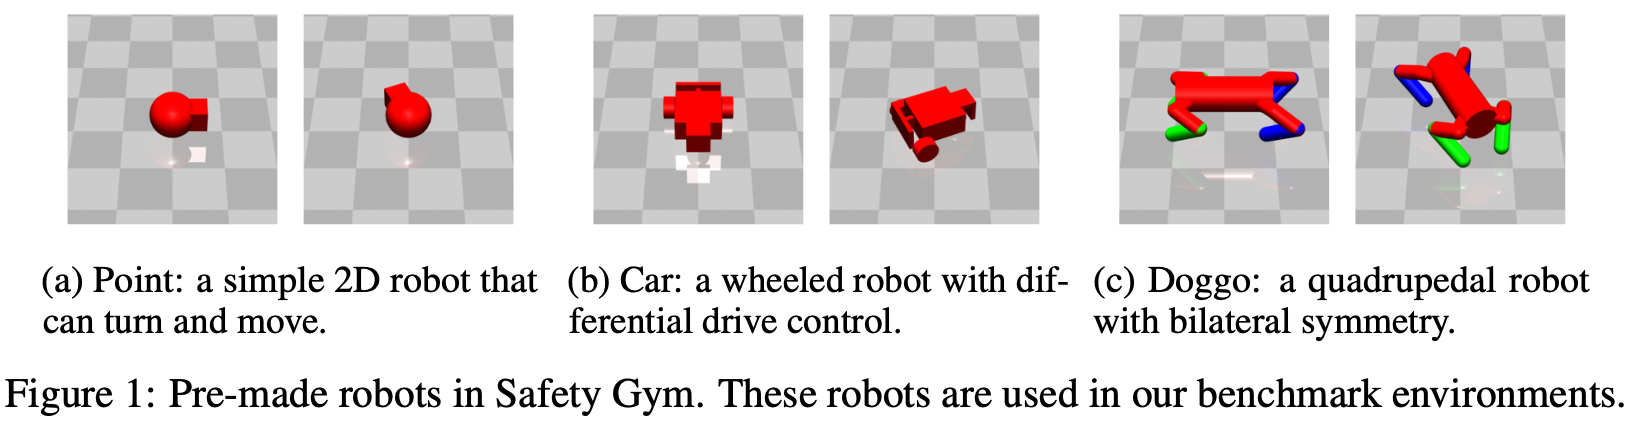
\includegraphics[width=0.7\textwidth]{./pics/robots.png}
    \label{fig:doggo}
\end{figure}

\textbf{Tasks} include Goal (move to a series of goal locations), Button (press a series of buttons), and Push (move a series of blocks). Reward functions could be sparse or dense. A demo figure from the paper \cite{ray2019benchmarking} is shown below:

\begin{figure}[h]
    \centering
    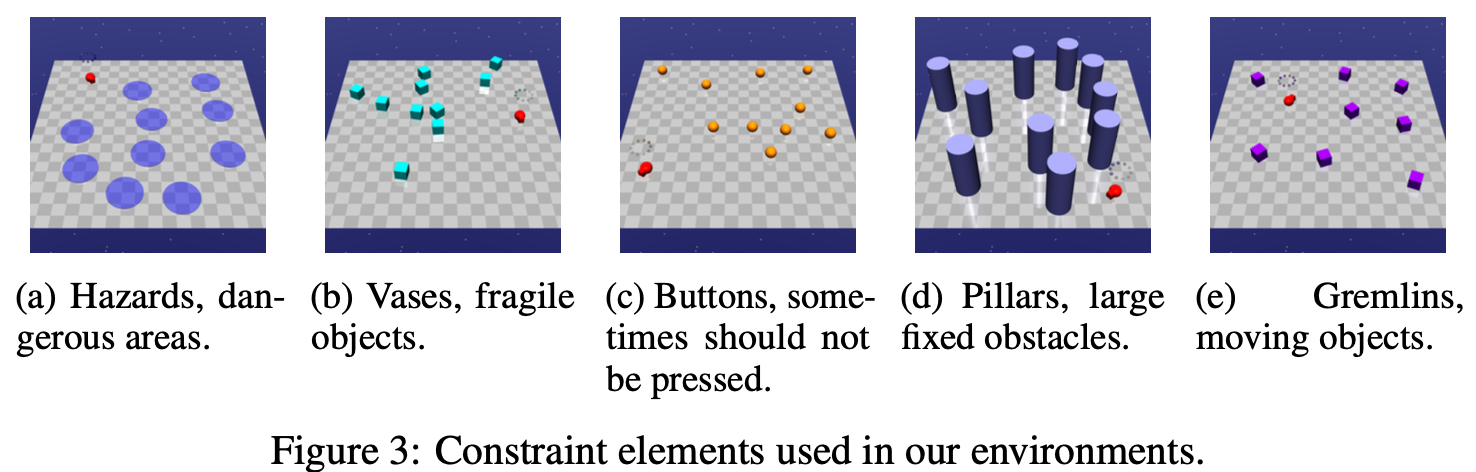
\includegraphics[width=0.7\textwidth]{./pics/tasks.png}
    \label{fig:tasks}
\end{figure}

\textbf{Constraint options} include: Hazards (dangerous areas), Vases (objects to avoid), Pillars (immobile obstacles), Buttons (incorrectly goals), and Gremlins (moving objects).

\textbf{Observations space options} are highly configurable, including: standard robot sensors, joint position and velocity sensors, compasses for pointing to goals, and lidar.

Lastly, users may enable \textbf{layout randomization}. Additionally, the \textbf{Safety Gym Benchmark Suite} serves as a zero-shot evaluation tool to assess the generalization performance of RL algorithms.

\section{Summary of Major Results}

The experiments evaluate several RL algorithms (mentioned before) on Safety Gym environments. Key results are summarized below:

\begin{itemize}
  \item Unconstrained RL gets high returns but violates safety.
  \item Constrained RL lowers returns to stay safe.
  \item Level 2 tasks are harder with more hazards.
  \item CPO fails to satisfy constraints; Lagrangian works better.
  \item Doggo learns with standard RL, but constrained RL fails.
\end{itemize}

\section{Summary of Strengths}

The paper provides a comprehensive but brief overview of the safety problem in AI, including the definitions, algorithms, and benchmarks. The authors also provide a clear motivation for using constrained RL for safe exploration. Moreover, the Safety Gym benchmark suite is well-designed and following the popular OpenAI Gym format, making it easy to use. 

\section{Summary of Weaknesses}

The Safety Gym community is barely active. While Gym is among the top three most popular OpenAI repositories with 36k stars, Safety Gym is much less popular, ranking 87th with just over 500 stars. More importantly, whereas Gym has over 1,700 commits and 300 contributors, Safety Gym has only 1 commit and is already archived. This indicates that Safety Gym is not widely used or researched.

However, there is a successor of Safety Gym called Safety Gymnasium by \citet{ji2023safety} published in 2023 with similar stars and more commits.

\section*{Acknowledgments}
This paper summary was independently conducted by the author Kunyi Yu. Meanwhile, the author would like to thank Professor Jiachen Li and TAs for their patient guidance and help.

\bibliographystyle{unsrtnat}
\bibliography{refs}

\end{document}
